\section{Цель работы}

Целью работы является экспериментальное исследование зависимости мощности теплового излучения от температуры, а также проверка закона Стефана–Больцмана.

Схема экспериментальной установки представлена на рис.~\ref{fig:setup}. В фокусе объектива \( O \) зрительной трубы пирометра расположена нить \( L \), изогнутая в форме полуокружности. Через окуляр \( O_{\text{ки}} \) с красным светофильтром \( \Phi \) наблюдатель видит среднюю часть нити на фоне поверхности тела, температуру которого требуется определить. 

С помощью потенциометра \( R \) осуществляется регулировка тока в нити и яркости её свечения. После включения нагрева кнопкой \( K \), ток, проходящий через нить пирометра, регулируется до тех пор, пока она не становится невидимой на фоне пластины.

Оптический пирометр прокалиброван по абсолютно чёрному телу. Шкала амперметра, измеряющего силу тока в нити, проградуирована в градусах Цельсия и определяет температуру нити, как если бы она являлась абсолютно чёрным телом.

\begin{figure}[htb]
    \centering
    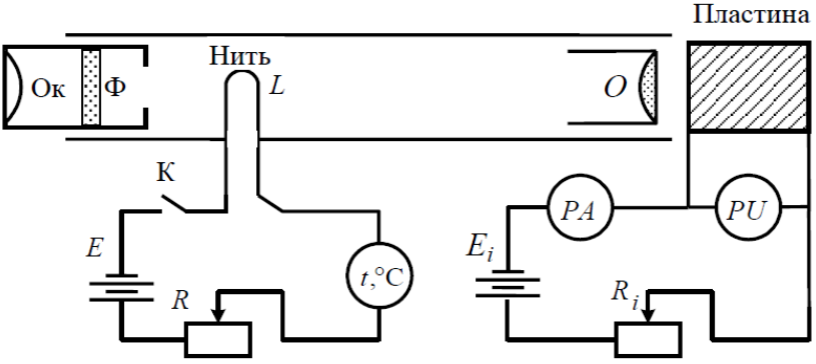
\includegraphics[width=0.7\textwidth]{images/ExperimentalSetup.png}
    \caption{Схема экспериментальной установки}
    \label{fig:setup}
\end{figure}

Электрическая схема нагрева пластины включает источник тока, амперметр \( P_A \) для измерения силы тока \( I \) в пластине, которая регулируется потенциометром \( R_i \), и вольтметр \( P_U \) для измерения напряжения \( U \), приложенного к пластине.
